\documentclass[a4paper,10pt]{article}
%\usepackage[utf8x]{inputenc}
%\usepackage{czech}
\usepackage[utf8]{inputenc}
\usepackage[czech]{babel}
\usepackage{graphicx}
\usepackage{subfig}

\title{Zpráva k~seminární úloze z~předmětu\\ Inteligentní robotika \\ {\small Závěrečná zpráva}}
\author{Filip Jareš, Lenka Mudrová}
\date{27.4.2011}

\begin{document}

\maketitle
\begin{figure}[!h]
	\centering
	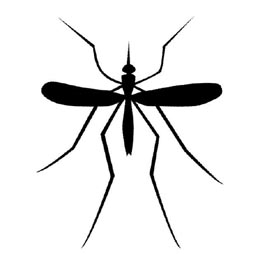
\includegraphics[width=0.4\columnwidth]{pics/mosquito}
	%\caption{}\label{fig:m}
\end{figure}
\newpage

\section{Popis úlohy}
		Řešená úloha je inspirována článkem Backyard star wars \cite{zadani}, který se zabývá problémem
		detekce komára ve venkovním prostředí a jeho sestřelení laserovým paprskem. 
		Pro školní účely byla tato myšlenka pozměněna, komár je nahrazen černým čtvercem, který se pohybuje na bílém
		pozadí monitoru, namísto laseru je pouze sledován kamerou.

		Poloha kamery se ovládá s použitím dvou modelářských serv a to  
		natočením okolo svislé osy (změnou azimutu) a natočením okolo vodorovné osy (změnou elevace). Cílem úlohy
		je řídit kameru tak, aby sledovala pohyb komára a zdokumentovala jeho „sestřel“
		sérií snímků, ve kterých je komár ve středu obrazu z~kamery – uprostřed
		„záměrného kříže“.

		

\section{Rozbor problému}
		Úloha se skládá z~několika oblastí, především je zde zastoupena oblast
		po\-čí\-ta\-čo\-vé\-ho vidění, kdy je nutné sejmout obrázek z~kamery, zpracovat ho a
		detekovat v~obraze komára. 
	        Další oblastí, která je zastoupena, je řízení. Celý
		program tvoří zpětnovazební regulační smyčku.
		V~neposlední řadě je v~problému zastoupena robotika, kdy je potřeba pracovat se
		soustavou serv a počítat transformace souřadnic mezi obrazovkou a souřadným
		systémem serv.

		\subsection{Popis konstrukce soustavy}
		Použitá soustava je tvořena LCD monitorem s poměrem stran $4:3$ a kamerou umístěnou na pan-tilt jednotce \cite{kamera} .
		Obrázek \ref{fig:soustava} znázorňuje vzájemné umístění monitoru a kamery.
		Pan-tilt jednotka je tvořena dvěma modelářskými servomechanismy, které umožňují pohyb mezi $x-y stupni$.
		% FIXME: To je divná formulace s těmi x-y stupni. Raději popsat/zmínit osy rotace?
		%TODO: udelat obrazek

	       \subsection{Popis kamery a ovládání}
	       %TODO: popis

	       \subsection{Popis servo mechanismu a ovládání}
		%TODO: popis? Tady jen popsat tu jejich funkci nebo? Nejak nevim

\section{Změny specifikace}

		%TODO: vymyslet to
		Oproti specifikaci úlohy v první zprávě jsme se rozhodli neimplementovat predikci letu komára 
		a to z důvodu, že testy prokázaly, že dobře naladěný PI regulátor reguluje pozici komára s dostatečnou 
		přesností 
		
\section{Řešení problému}

		\begin{figure}[!h]
			\centering
			 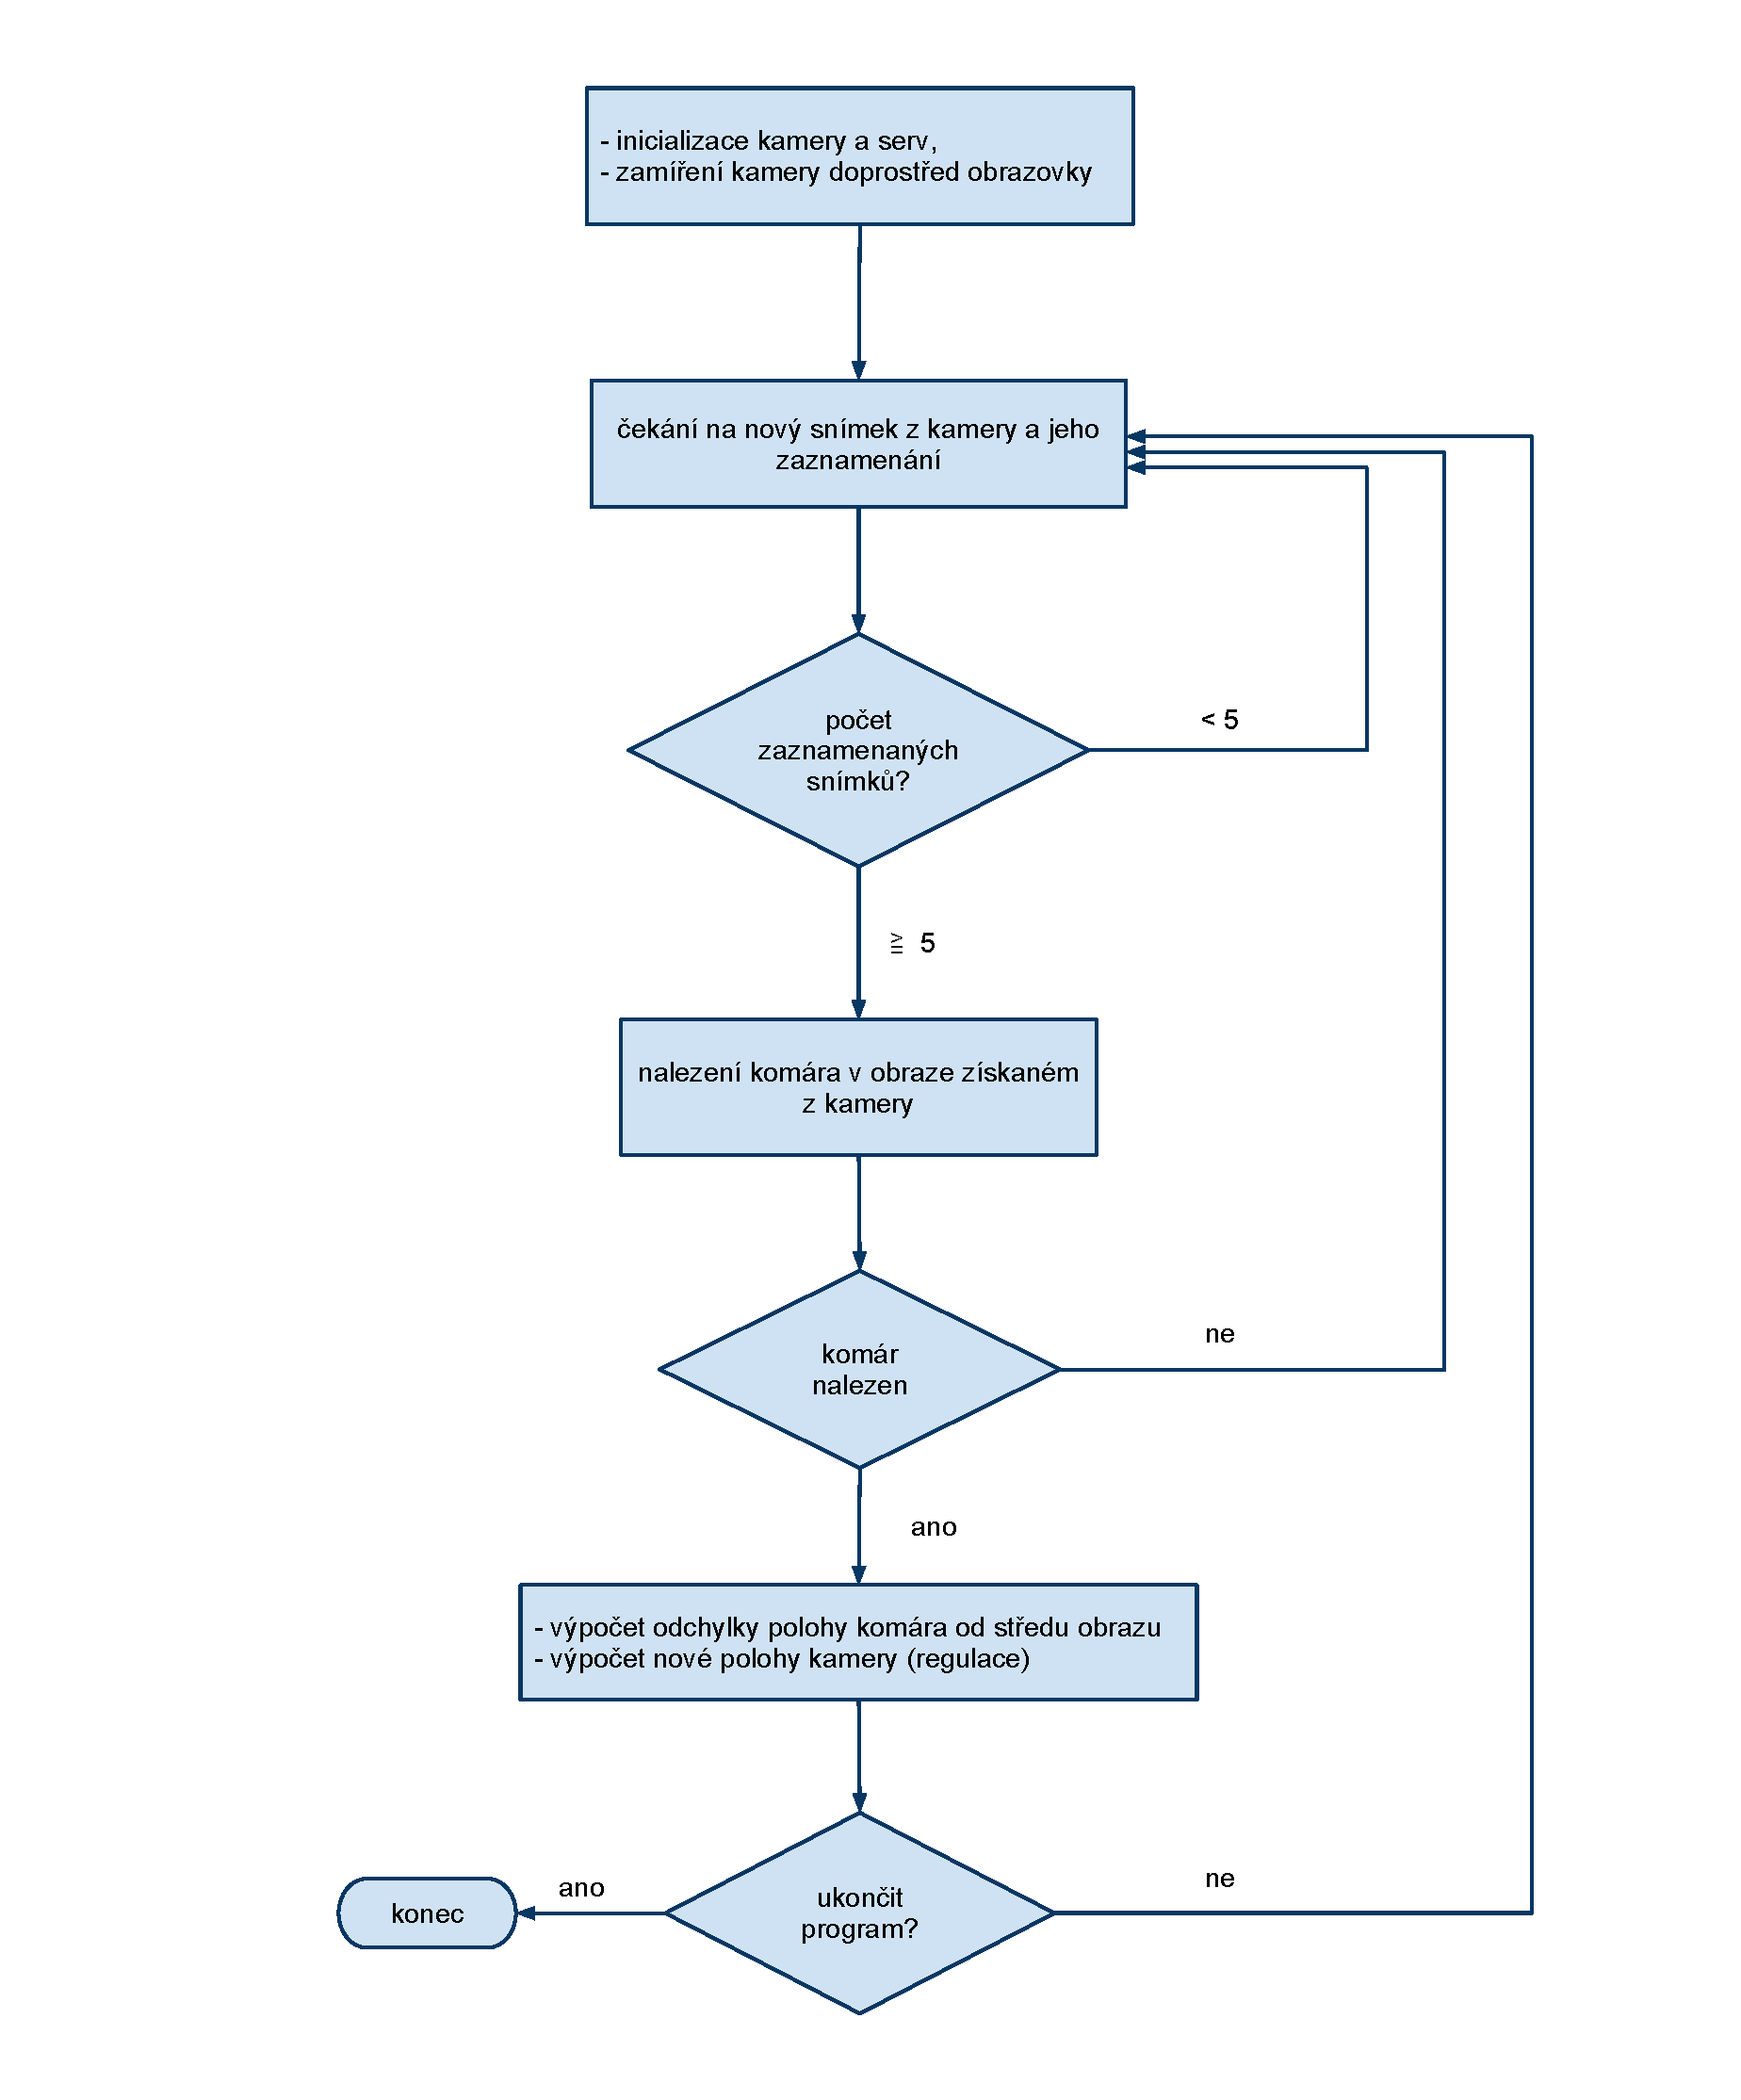
\includegraphics[width=1\columnwidth]{pics/vyvojovy_diagram_programu}
			 \caption{Vývojový diagram programu}\label{fig:Diagram_programu}
		\end{figure}



		Program se spouští hlavní funkcí \textit{startMosquitoHunter}. 
		Nejprve se zincializuje kamera a servo mechanismy. 
		Následně se kamera nastaví na střed obrazovky, kde se vyčkává příletu komára do zorného pole kamery. 
		Tato funkce volá s~využitím callback funkce výkonou funkci \textit{processNextFrame}, která zahrnuje hlavní chod
		programu. Perioda spouštění je nastavena na dvojnásobek snímací frekvence, k~regulaci se používá každý druhý obrázek.
		%TODO: proc se bere kazdy druhy?

		Funkce \textit{processNextFrame} pracuje s~jedním obrazem získaným z~kamery, vybere z něj pouze zelenou složku.
		Pro použití jedné složky jsme se rozhodli především proto, že oproti debayerizaci je výpočetně nenáročná a 
		umožňuje v paměti uchovávat více obrázků. Pro zelenou složku jsme se rozhodli na základě pozorování, 
		jelikož poskytuje největší kontrast oproti ostatním barevným složkám.

		Takto upravený obraz se předá funkci \textit{findMosquitoInImage} a 
		následně je porovnán s~empiricky určeným prahem.
		Tím vznikne binární maska s~oblastmi, které vykazují barevnou podobnost s~hle\-da\-ným komárem, viz obr. \ref{fig:komar_obr3}.

		\begin{figure}[!htb]
		  \subfloat[\label{fig:komar_obr1}]{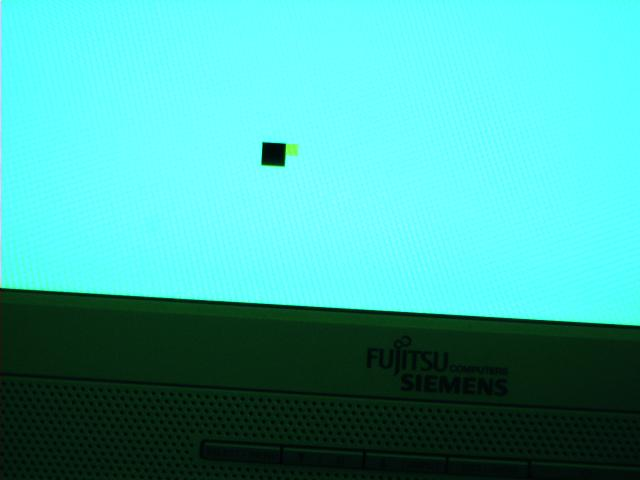
\includegraphics[width=0.49\columnwidth]{pics/zpracovani_obrazu-1.jpg}}
		  \hfill
		  \subfloat[\label{fig:komar_obr2}]{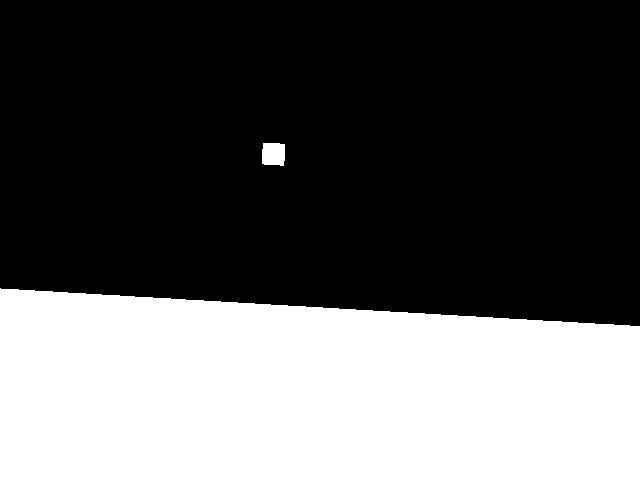
\includegraphics[width=0.49\columnwidth]{pics/zpracovani_obrazu-2.jpg}}
		  \caption{Nasnímaný obrázek a binární maska}
		\end{figure}
		
		\begin{figure}[!htb]
		    \subfloat[\label{fig:komar_obr3}]{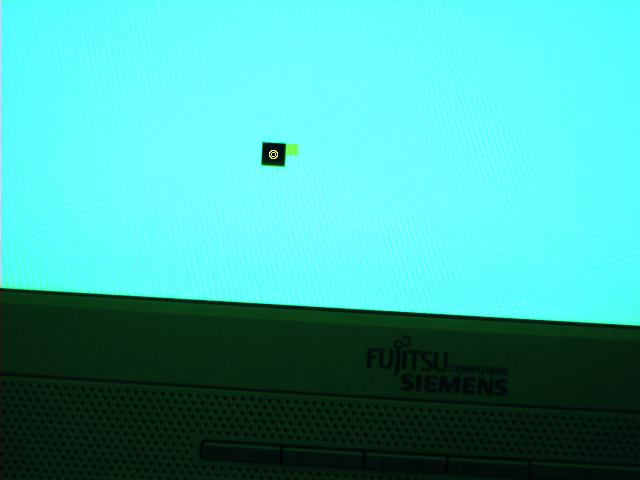
\includegraphics[width=0.49\columnwidth]{pics/zpracovani_obrazu-3.jpg}}
		    \hfill
		    \subfloat[\label{fig:komar_obr4}]{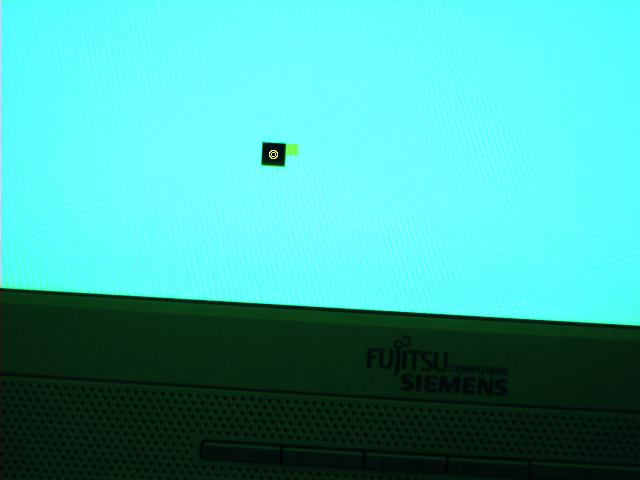
\includegraphics[width=0.49\columnwidth]{pics/zpracovani_obrazu-3.jpg}}
		    \caption{Souvislé oblasti s parametrem plocha a hlavní osa; komár se středem}
		\end{figure}
		
		K~získání polohy komára v~obrazu z~kamery byl použit jednoduchý algoritmus
		využívající morfologických funkci Matlabovského Image Processing Toolboxu. 
		V~binární masce jsou nalezeny souvislé oblasti využitím funkce \textit{bwlabel}.
		Z~těchto oblastí je vybrána ta, kterou považujeme za komára. Pro toto
		rozhodnutí jsou použity vlastnosti oblastí \textit{MajorAxisLenght} a
		\textit{Area}. Jsou vyloučeny takové oblasti, jejichž plocha je větší než $3000$
		pixelů nebo jejichž délka je více než $50$ pixelů. Tyto hodnoty byly nastaveny
		na základě maximálních parametrů komára a dostatečné rezervy. Ze zbývajících
		oblastí je vybrána ta, která má největší plochu. Pro tuto oblast je určena
		poloha středu v~pixelových souřadnicích a tato infromace je návratová hodnota
		funkce \textit{findMosquitoInImage}. 
		Tyto hodnoty jsou předány funkci \textit{mosquitoPxPositionToAzimuthAndElevation},
		která vypočte hodnoty azimutu a elevace. 

	        Regulace, tedy výpočet nové polohy kamery $x_{new}, y_{new}$, je řešena jako PI
		regulátor v~těle funkce \textit{processNextFrame}. 
	        Vypočte se rozdíl mezi skutečnou a žádanou hodnotou $err$ a do
		proměné $sum_e$ se tato odchylka přičítá, při čemž její počáteční hodnota je
		nulová. Proměné $x, y$ jsou souřadnice aktuální polohy kamery.

		$$x_{new} = x + P\cdot err + I\cdot sum_e$$
		$$y_{new} = y + P\cdot err + I\cdot sum_e$$

		Pozice kamery je saturována na hodnoty, ve
		kterých je očekáván komár, tedy na hodnoty odpovídající kraji monitoru.

		Konstanty $P$ a $I$ jsou naladěny pro každý směr zvlášť, byl implementován antiwind-up jev.
		



%Funkce \textit{processNextFrame} tvoří zpětnovazební regulační smyčkou pro řízení polohy
%		kamery. Vstupem regulátoru je nejnovější získaný obrázek z~kamery a jeho
%		výstupem je nová poloha kamery.


%Před samotným výpočtem nové polohy kamery
%		je vyhodnocen nově zís\-ka\-ný obraz. Postup jeho zpracování je znázorněn na
%		obrázku~\ref{fig:zpracovaniObrazu}.  Nejprve je určena poloha komára v~obraze
%		(funkce \textit{findMosquitoInImage}) v~pixelových sou\-řad\-ni\-cích. Na základě odchylky
%		této polohy od středu obrázku potom funkce
%		\textit{mos\-quito\-Px\-PositionToAzimuthAndElevation} počítá odhad úhlů, o~které je
%		komár vy\-chý\-len od optické osy kamery. Pro urychlení celé smyčky jsou data pouze
%		ukládána, nikoliv zobrazována. Uživatel si snadno tato data přehraje offline.


\section{Implementace}

		

		

\section{Experimentální výsledky}

\section{Diskuze a Závěr}

\bibliographystyle{splncs03}
\bibliography{report}

\end{document}
 
